\documentclass[11pt]{article}
\title{%
\Huge Empirical Analysis\\
\color{white} blank line\\
\color{black}
\Large
Using recursive backtracking\\
on Peg Solitaire}
\date{2017}
\author{Lindiwe Mncwabe - 1118055\\\\Clifford Ralikhwatha - 0412610\\\\Thomas Johannsen - 721988\\\\\\\\}

\usepackage[margin=1.2in]{geometry}
\usepackage{hyperref}
\usepackage{graphicx}
\hypersetup
{
    colorlinks=true,
    linkcolor=blue,
    filecolor=magenta,      
    urlcolor=blue,
}

\begin{document}
\maketitle
\pagenumbering{gobble}
\newpage
\tableofcontents
\listoffigures
\newpage
\pagenumbering{arabic}
\section{Introduction}
\subsection{Overview}
This project is a joint effort by the above authors to perform empirical analysis on our algorithm that solves various peg solitaire boards. The algorithm reads in the initial game board and the goal state and then proceeds to solve the board by means of a recursive backtracking algorithm. Due to complexities discussed later, we implemented a hash table to stored previously checked board states to speed up the process.
\subsection{Aims}
The aim was to write an algorithm using Java, that would solve the classic peg\\ solitaire board in a reasonable time. Once the basic functionally was working the next goal was to solve additional boards, of various shapes and sizes, to compare how the algorithm performs.\\
\newpage

\begin{figure}
\section{Peg Solitaire}
Peg solitaire is a very old single player game, that is played on a board of 33 holes in a cross formation. The aim is to jump pegs/marbles/stones over each other, removing one in the process, until just a single peg is left in the centre of the board. Different variations exist, some that use more than the standard 33 pegs, others that use less.\\
Figure 1 shows an example of a valid move.\\\\
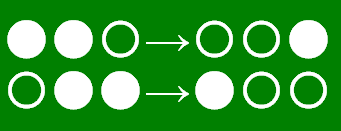
\includegraphics[width=5cm]{1}
\caption{Example of a move} 
\label{fig: 1}
\subsection{Theory}
\subsubsection*{The Game}
It soon becomes clear that the game is mathematically very complex. The first move has 4 possibilities, each of those 4 moves has its own 4 possibilities. From this we can extrapolate that the number of possibilities grows at the rate$(O^4)$, in actual fact its less than that, due to not all 4 possibilities always being valid moves and many of them resulting in the same board state. None the less the problem grows at an exponential rate.\\
The exact number of different sequences for the game is $5*10^{20}$~\cite{durango},  $4*10^{16}$ of these are solutions. It turns out that all of those solutions are rotations and symmetries of one unique sequence. 
All solutions use exactly 31 moves, by the design of the game a move removes a peg, so no solution is better or worse than any other.

\subsubsection*{Recursion}
Recursion can be a risky concept to implement, the idea is that the functions at some point calls itself, this can very easily result in an infinite loop. The reason we can use it for this problem is that we can control the recursion. On each call of the function we remove a peg, that means that we cannot call the function more often than we have pegs. We only add pegs back onto the board when we step out of a function and return to a shallower depth of recursion.
\end{figure}
\begin{figure}

\subsubsection*{Backtracking}
As the name suggest, backtracking is a method that makes an initial guess and then tests if that guess was correct, if not we backtrack along the sequence traversed so far and try a different move. 
Applied to peg solitaire; once we reach a board state that isn't the final solution, but also has no possible moves left we know that we have made a mistake at some point, so we undo our last move. This is done by adding the peg that was removed back onto the board and then trying a different jump instead. Once all options have been exhausted we backtrack a step further.
\subsection{Design}
To begin we need to represent the board somehow. There are many way to do this, but we decided to store it as a 7x7 matrix, where a 0 represents out of bounds, 2 is a peg and 1 is a hole. It turns out that 1 and 2 are interchangeable because the reverse of the solution would be building the board from just 1 peg to a full board with a single hole in the middle. Well that is the exact same problem with the definition of 1 and 2 swapped. We set 1 and 2 as defined so that the final board state has a hash value of 0.
A sequence is considered a dead end, if we cannot perform any further moves and the board is not solved. Any solution we find is accepted, there is no need to find further solutions, as every solution has the same length.\\\newline
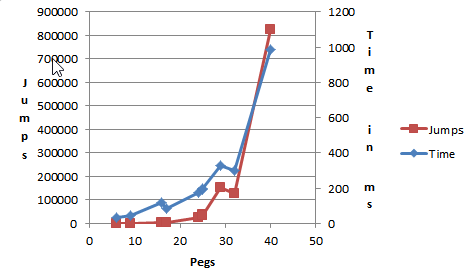
\includegraphics[width=15cm]{6}
\caption{Matrix of the solved board and flowchart of the pseudo code}
\label{fig:2}
\color{white} blank line\\
\color{black}
The algorithm runs through the matrix trying on every element to perform a jump, in the order left, up, down, right and then storing that move in a separate array. The function is then called again and the algorithm scans for the next possible jump. Once it has been determined that the sequence is a dead end, the board state is saved to the hash table and we backtrack one step to a shallower recursion level. Here we try to jump from the same position, but into a different direction, if possible, otherwise we scan for the next element on which we can perform a jump.
\end{figure}
\newpage
\begin{figure}
\subsubsection*{Proof of Correctness}
The algorithm is a depth first recursive algorithm, with backtracking. To speed up the process we prune dead branches. By the nature of it being depth first it will scan every possible move. This guarantees that we find a solution, if the board is solvable. We can be sure that the pruning doesn't skip any untested moves, as it only stored boards that have been exhausted. 
If we look at figure 3, we search to the left of the root node, till we can't any more. We get to (5), this isn't the solution, so we save the current board state to the hash table and backtrack to (4), proceeding in a different direction than we took to (5), this leads to (7). This is also not the solution, so we save the hash and backtrack, repeating the procedure till we return to (4), which has not been exhausted and is therefore hashed. 
Backtracking further to (3), we try a direction that didn't lead to (4), but when we check the hash value of the board at (8) we see that it is the same as at (4), so we skip the entire branch, as it can't be solved. We try a different direction from (3), or backtrack to (2).
\newline\\
\includegraphics[width=5cm]{3}
\caption{Depth First Search} 
\label{fig: 3}
\subsubsection*{Hash Table}
The idea behind the hash table was to store boards that have already been checked, as in many cases doing jump A and then jump B has the same result as B then A. If we know that AB doesn't yield a result, there is no need to run through the branch of BA.
Due to the high level of symmetry in the board, we decided that not only should a branch be pruned if it has a dead end board state, but also if the board state is a rotation of a dead end state. 
\end{figure}
\newpage
\begin{figure}
\subsubsection*{Design 1}
The first idea for the hash table was that every element of the matrix has a unique value assigned to it. We include all 49 element of the matrix, in case we want to test a board that uses a different shape from the standard cross. Out of bounds elements and elements with no pegs are considered 0 and a peg is considered a 1. This results in a 49 bit binary hash value. We considered two possible ways to compare the hash values of rotated board states. First rotating the matrix by multiplying by a rotation matrix and then hashing it, or identifying the pattern in the hash value, as all elements are rotated to a different element we rearrange the hash value.
Both of these methods seemed a bit cumbersome so we came up with design 2 instead.
\subsubsection*{Design 2}
Instead of using 49 unique values we mapped and colour coded the symmetries of the board. Each element has 4 or 8 equivalent positions, we sum these positions and multiply each by a different power of 10, to obtain a value that is unique to that board state and its congruent siblings.\\
Figure 3 shows the design of the hash map we ended up using. The central piece is the only one with no symmetries, so we store it as a boolean, by making the hash positive or negative depending on whether it has a peg or not.
\newline
\color{white} blank line\\
\color{black}
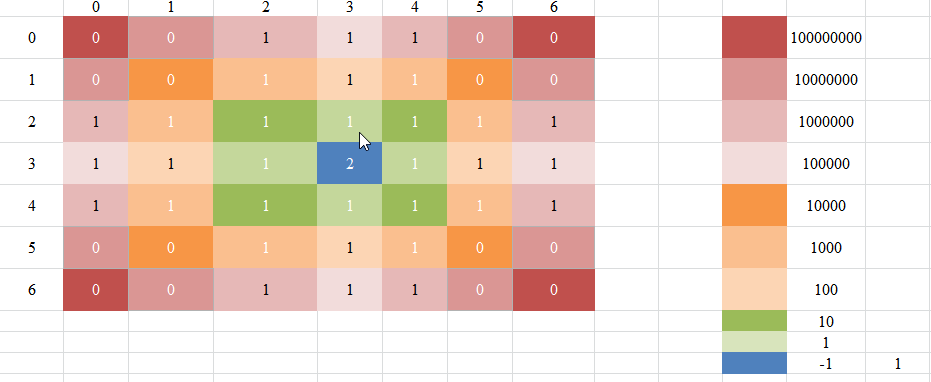
\includegraphics[width=\textwidth]{4}
\caption{Colour coded hash map} 
\label{fig: 3}
\end{figure}
\newpage

\begin{figure}
\subsection{Experimentation}
The first draft of the algorithm didn't make use of the hash table. We read in the start board and starting performing jumps and backtracking and let that run for a while.
It found the 29th jump after trying 10 000 jumps, and the 30th after 90 000 but 30 hours and over 100 billion jumps later, it hadn't found the last move to solve the problem.\newline
It was clear that this was far too slow, even worse we had no way of predicting how long it would take to find the final move to solve the problem. It could at any stage be the next jump, or it could still be hours away. Considering how many possibilities there are in total we thought it was unlikely that we would find the solution any time soon. We should instead try optimise the search, find a way to make it smarter or faster.\\
First we found that a minor change to the order of the jumps can make a difference. Initially we had: right, left, up, down, but it turns out that if the first 2 jumps are opposite directions it takes a lot longer than if they are 90$^{\circ}$ rotations. Which direction is chosen as first or second... makes very little difference due to the symmetry of the game.\\
We wanted to half the search depth, by trying to solve the problem from both sides, 1 algorithm that starts from the beginning and another that starts from the solution and they work towards each other and meet at the middle.
We weren't quite sure how to implement this, so we started doing some research and came across the work of Masashi Kiyomi and Tomomi Matsui~\cite{Tomomi}.
They use three different optimisation methods, the first is to set up the problem as a integer problem and solve the feasibility of that at each step, as we don't know much about integer problem solving we skipped this.\newline
The next two points they make are to use a hash table to avoid repetition and solving forwards as well as backwards. The last two ideas were similar to our ideas, so we decided to spend some time thinking how we would implement them.\newline
We decided not the split the problem in half, and just solve it as is, as we couldn't come up with a good idea on how to store each board state, considering that if a later recursion of the one meets an earlier recursion of the other, we would need to store the moves performed getting to that board. This means storing not only the hash value of half depth board states, but also the moves to get to them.

\end{figure}
\newpage
\begin{figure}
\subsection{Results}
The hash table showed incredible improvements, so much so that we decided we didn't need pursue the integer problem method.\\
At first we were storing hash values randomly and repeatedly in the hash table, but still cut the execution of the problem to 4.6 seconds. Once we started trying bigger boards (40+ pegs), the run time sky rocketed, because the hash table grew with every jump tried. Very soon the lookup in the massive table resulted in the coded being slower than before.
We then opted to store the hash values in a red-black tree, so that they remain sorted and unique, for faster looking up.
This cut the time to 200ms and reduced the number of hash values by about 30\%, while improving look up from linear to log(n) time.\newline
As we will show, there are three important details to be considered for a run time execution of a board.
\begin{itemize}
\item The number of starting pegs
\item The shape in which the pegs are set up
\item The number of out of bounds fields
\end{itemize}
Unfortunately we can't directly compare all of these, as not all designs are solvable. This means that an unsolvable board with the same amount of pegs as a solvable board will result in many many more jumps, because the algorithm only ends once every branch has been exhausted.\newline
We designed some different shapes, with different number of starting pegs, ran them, and plotted the outcome.\\
\color{white} blank line\\
\color{black}
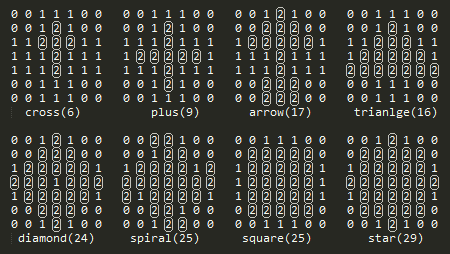
\includegraphics[width=12cm]{5}
\caption{Different Starting Boards} 
\label{fig: 5}
The hash table made no difference at all for small boards, cross and plus cross, on the number of jumps or the run time.\\
For all bigger boards it's not even worth running without the hash table, they takes minutes or hours to solve.\\
\end{figure}
\newpage

\begin{figure}
Figure 6 shows the number of pegs plotted against the number of jumps and the run time till the solution is found or all moves have been tried.\newline
\newline
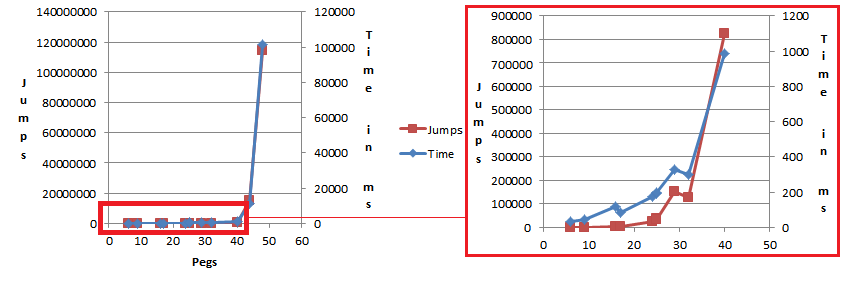
\includegraphics[width=15cm]{7}
\caption{Graph of results} 
\label{fig: 6}

\subsection{Interpretation}
The first thing that should be noted about the graph is that the 40+ peg boards were not solvable. This means that the algorithm terminates sooner on all other boards, as it just finds the first solution, opposed to running to conclusion which is the case for the 40+ peg boards.\\
We feared this might skew the graph a bit, and we considered leaving out the 40+ peg boards from it. But first we decided to investigate on the magnitude of the difference between finding the first solution and running to conclusion. We reran the smaller boards with unreachable goal states, to force the algorithm to exhaust every possible sequence, the runtime difference was so minute that it wouldn't even show on the graph. This is because of the total amount of possible sequences only a tiny fraction are solutions, by the time a solution has been found the majority of sequences have been check, so checking the remaining few after the initial solution is relatively quick. Keep in mind that we don't need to check all possible sequences, as the hash table eliminates rotations, greatly reducing the total possible sequences.\\
The exponential nature of the graph is clear, bigger boards have longer sequences and also have more possible jumps at each step to be considered, and therefore take longer to solve.\\
If we look at the zoomed in part of the graph we notice two points that don't lie on the curve, those are at 16/17 and 29/32.\\
If we look back to figure 5, we see that 16 pegs is the triangle, which has 12 possible first moves, 17 pegs is the arrow, which only has 8 starting moves. The arrow also has 2 groups of pegs joined by a single line. Even though the triangle has less pegs it has more possible jumps to consider at every step.\newline
If we look at the next disturbance, we have 29 pegs, the star, and 32, the classic board. The star has a bigger playable board, because the standard board has 16 elements out of bounds and 33 playable fields, while the star has 12 out of bounds and 37 playable elements. This results in the star being the more complex puzzle, as at any given stage there are more possible jumps to consider.\\
\end{figure}
\newpage
\begin{figure}
For 25 pegs we found two separate solvable boards, the spiral and the square. Their run time is almost identical, as the jumps to completion differs by about 200 (35540 and 35332). This surprised us, as the square has 12 out of bounds compared to the 16 of the spiral, so we expected the square to take longer. Although if we count the possible starting moves the square has 12 to the 16 of the spiral. The two differences counteract each other and almost perfectly cancel out in this case
\newline.
\newline
The trend is clear though that as the number of pegs increase the solution takes exponentially longer to find, with the shape causing some minor variance from the trend.

\section{Conclusion}
With a problem of this nature it is hard to predict how well an algorithm will perform. From our empirical data we can see that the trend of the graph is exponential, which is what we expected. It is quite remarkable what an improvement the hash table made.

\end{figure}

\newpage
\begin{figure}

\bibliographystyle{plain}
\bibliography{MyBibFile}
\end{figure}
\end{document}